    In this case,
    \begin{align}
	    \vec{B}-\vec{A} &=  \myvec{3\\3\\3} \\
	    \vec{M} &=  \myvec{1&2\\-3&3\\2&1}. 
                \label{eq:chapters/12/11/2/16/given}
    \end{align}
	    forming the matrix in \eqref{eq:chapters/12/11/2/16/lsq/rank},
    \begin{align*}
        \myvec{1&2&3\\-3&3&3\\2&1&3} \xleftrightarrow[]{R_2\leftarrow R_2+3R_1} \myvec{1&2&3\\0&9&12\\2&1&3} \\
                \xleftrightarrow[]{R_3\leftarrow R_3-2R_1} \myvec{1&2&3\\0&9&12\\0&-3&-3} %\\
                \xleftrightarrow[]{R_3\leftarrow 3R_3+R_2} \myvec{1&2&3\\0&9&12\\0&0&3}
    \end{align*}
    Clearly, the rank of this matrix is 3, and therefore, the lines are skew.
%
        From \eqref{eq:chapters/12/11/2/16/lsq/vec-eqn},
    \begin{align*}
        \augvec{2}{1}{14&-5&0\\-5&14&18} \xleftrightarrow[]{R_1\leftarrow R_1+R_2} \augvec{2}{1}{9&9&18\\-5&14&18} \\
                 \xleftrightarrow[]{R_1\leftarrow\frac{R_1}{9}} \augvec{2}{1}{1&1&2\\-5&14&18} 
                 \xleftrightarrow[]{R_2\leftarrow R_2+5R_1} \augvec{2}{1}{1&1&2\\0&19&28} \\
                 \xleftrightarrow[]{R_1\leftarrow19R_1-R_2} \augvec{2}{1}{19&0&10\\0&19&28} 
                 \xleftrightarrow[]{\substack{R_1\leftarrow\frac{R_1}{19}\\R_2\leftarrow\frac{R_2}{9}}}
                    \augvec{2}{1}{1&0&\frac{10}{19}\\0&1&\frac{28}{19}} 
    \end{align*}
    yielding
\begin{align}
                    \bm{\kappa} = \frac{1}{19}\myvec{10\\28}
\label{eq:chapters/12/11/2/16/L2/svd/kappa}
\end{align}
        Substituting the above in \eqref{eq:chapters/12/11/2/16/L2/svd},
    \begin{align}
        \vec{x}_1 = \frac{1}{19}\myvec{29\\8\\77},\, \vec{x}_2 = \frac{1}{19}\myvec{20\\11\\86}.
    \end{align}
    Thus, the required distance is
    \begin{align}
        \norm{\vec{x}_2-\vec{x}_1} = \frac{3}{\sqrt{19}}
    \end{align}
See \figref{fig:chapters/12/11/2/16/skew}.
    \begin{figure}[H]
        \centering
        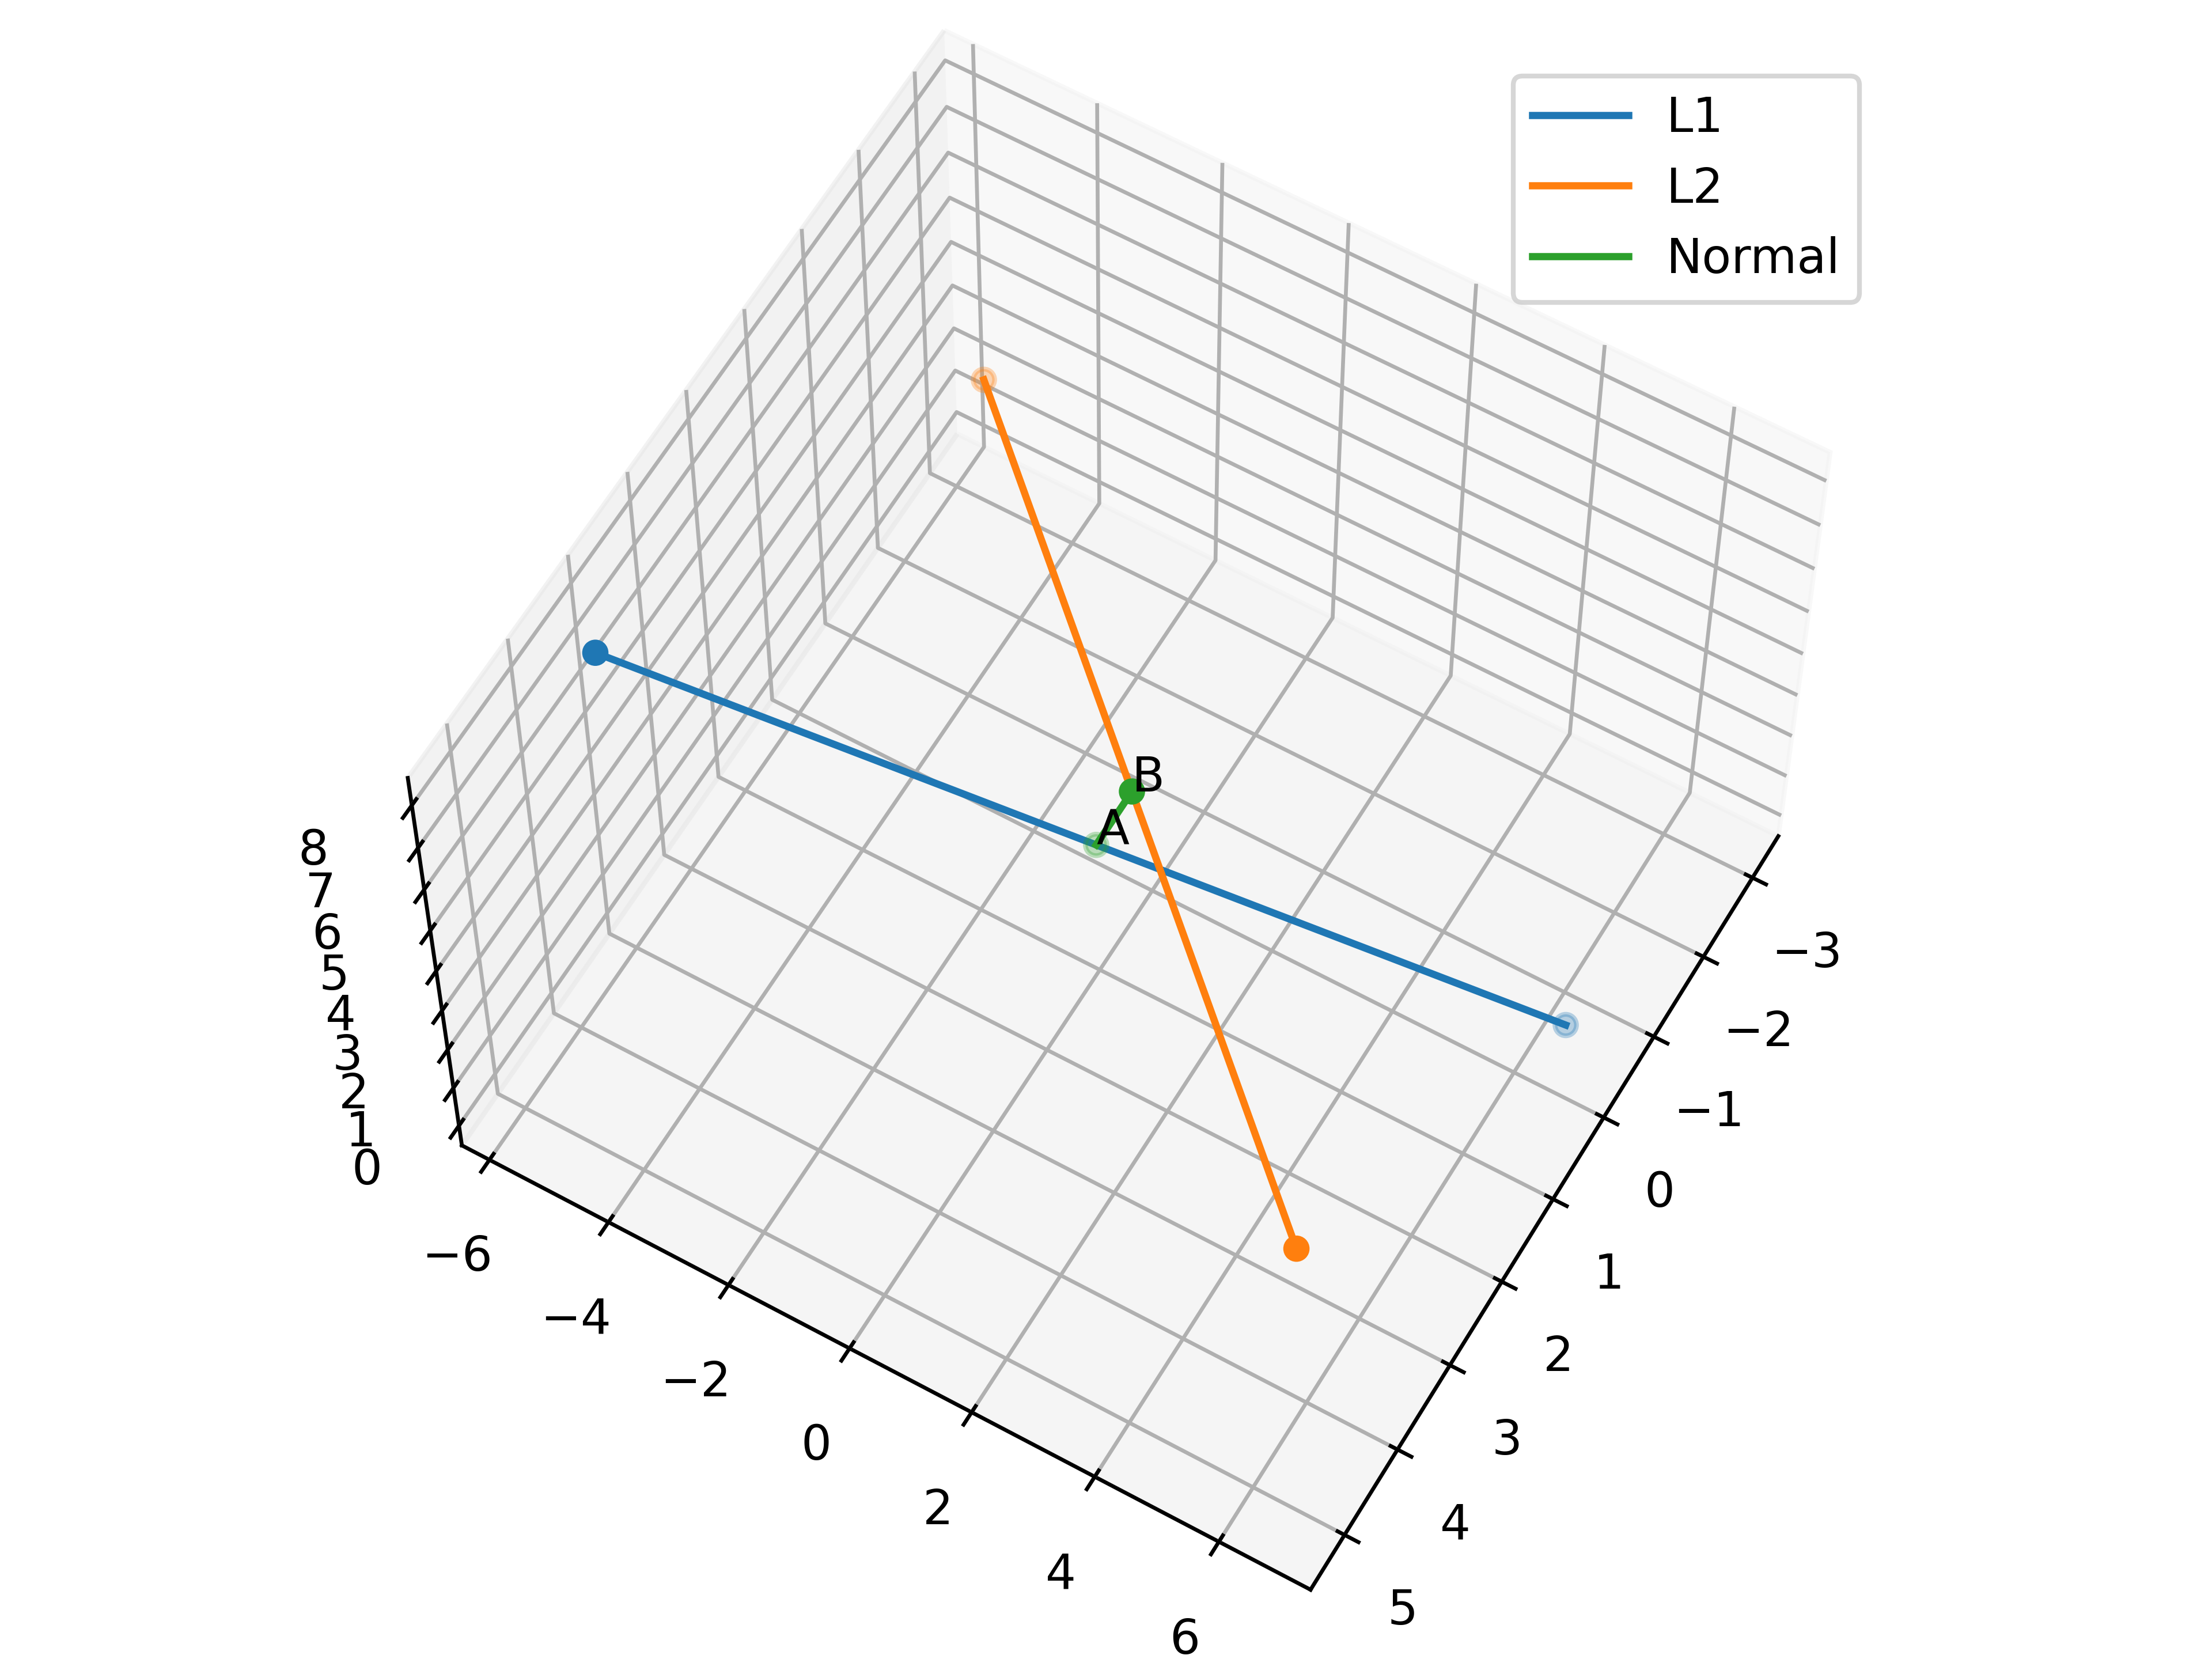
\includegraphics[width=0.75\columnwidth]{chapters/12/11/2/16/lsq/figs/skew.png}
        \caption{}
        \label{fig:chapters/12/11/2/16/skew}
    \end{figure}
